\section{Question 6 (Theorectial) and 5 (Simulation)-Frequency Response}
In this section, both octave and ngspice were used in order to obtain plots of the pahse response and of the magnitude response, using logscale. This approach is very useful hence it provides a much better plot fit and, therefore it provides great visualization for users. The magnitude in debicels is of interest for analysis of sound waves, and the analysis of the phase or angle delay is a very interesting way of study another parameter to compare signal. Frequency range in both analysis was from 0.1 Hz to 1MHz. The plots made were v6(f), vs(f) and vc=(v6(f)-v8(f)).
\subsection{Theoretical Analysis}

\subsection{Frequency Response- Magnitude}
\subsubsection{Frequency Response- Phase}







\subsection{Simulation Analysis}
In this part of the assignment, an AC (Small Signal Analysis was conducted, in order to match the goal aforementioned. This type of analysis allows to study the frequency response of the circuit. In other words, there is no frequency variation over time, the so called steady-state analysis.


\subsubsection{Frequency Response- Magnitude}

\begin{figure}[ht] \centering
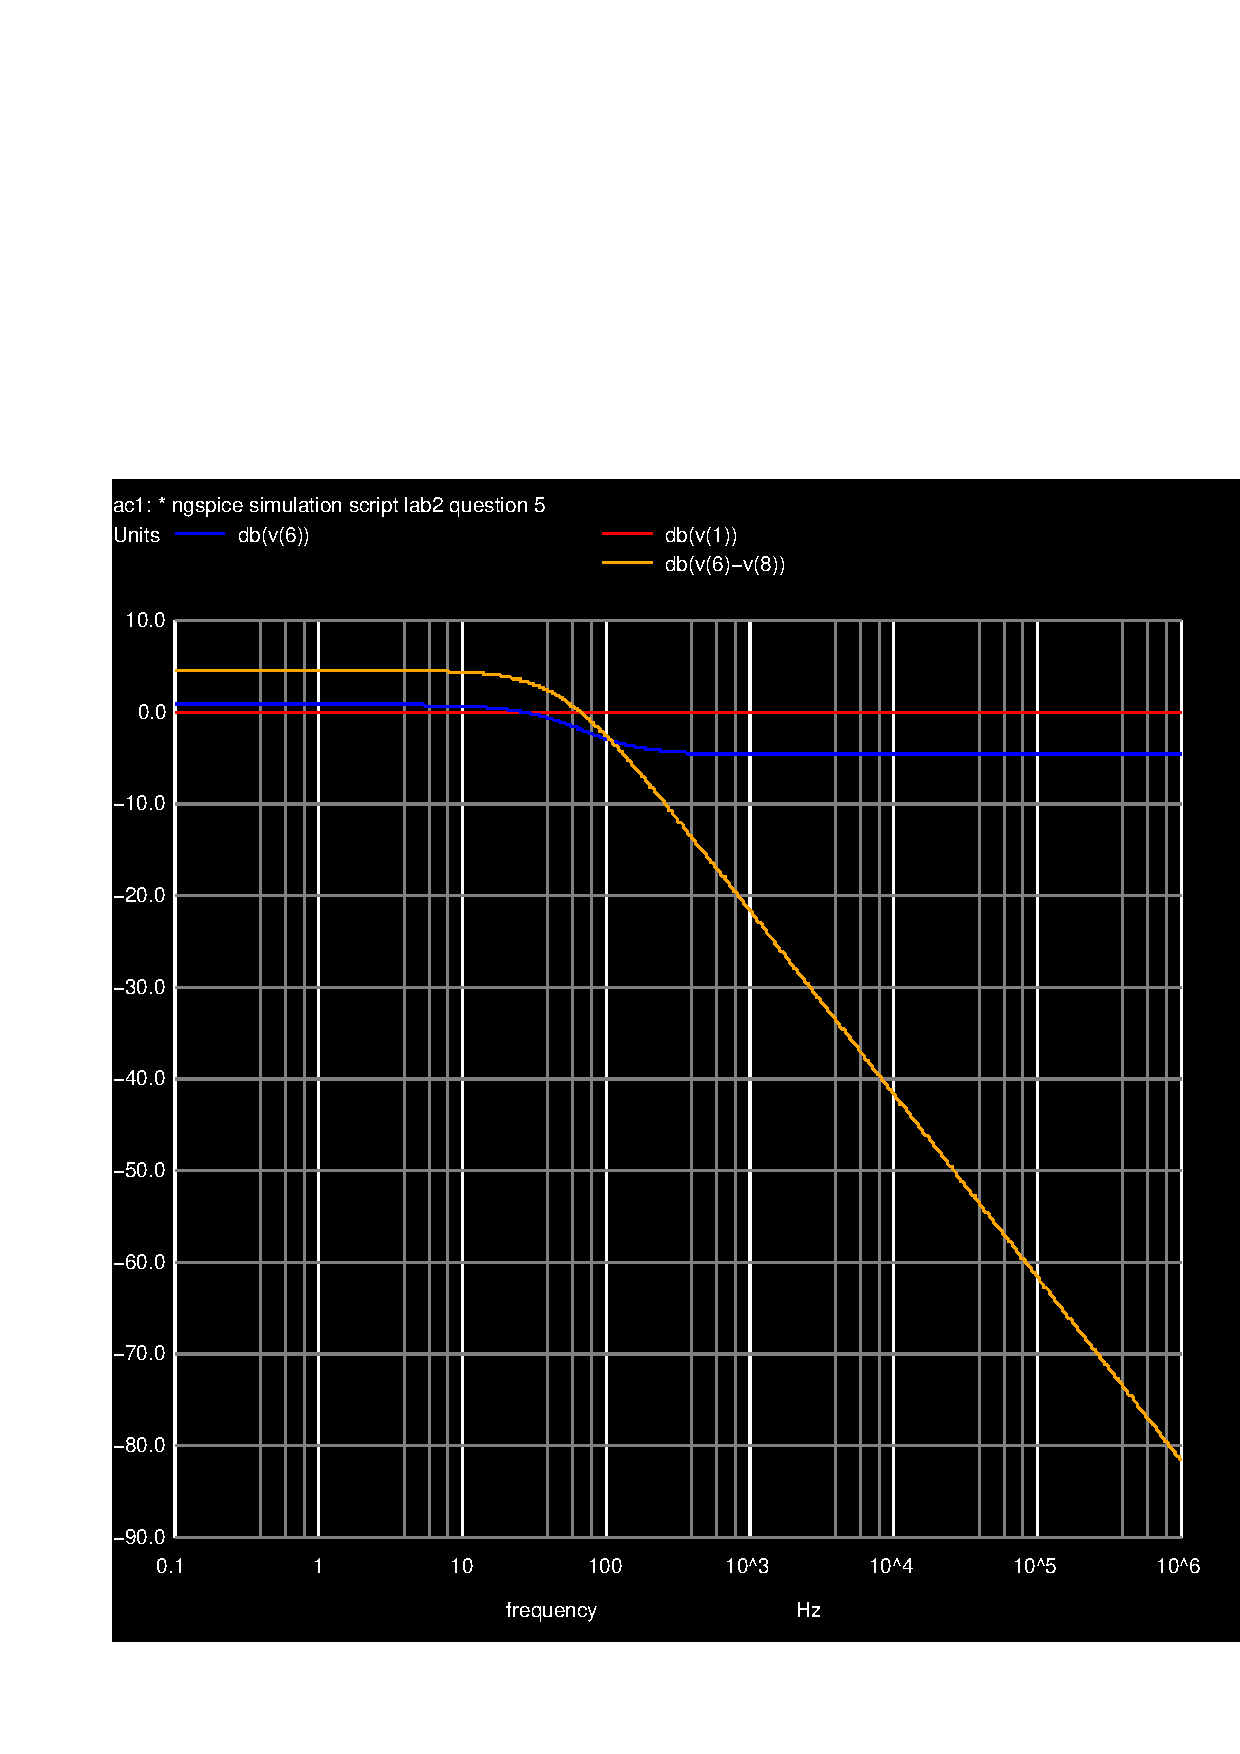
\includegraphics[width=0.9\linewidth]{sim5_db.pdf}
\caption{Magnitude Response (in decibels)}
\label{fig:sim5_db}
\end{figure}

\subsubsection{Frequency Response- Phase}

\begin{figure}[ht] \centering
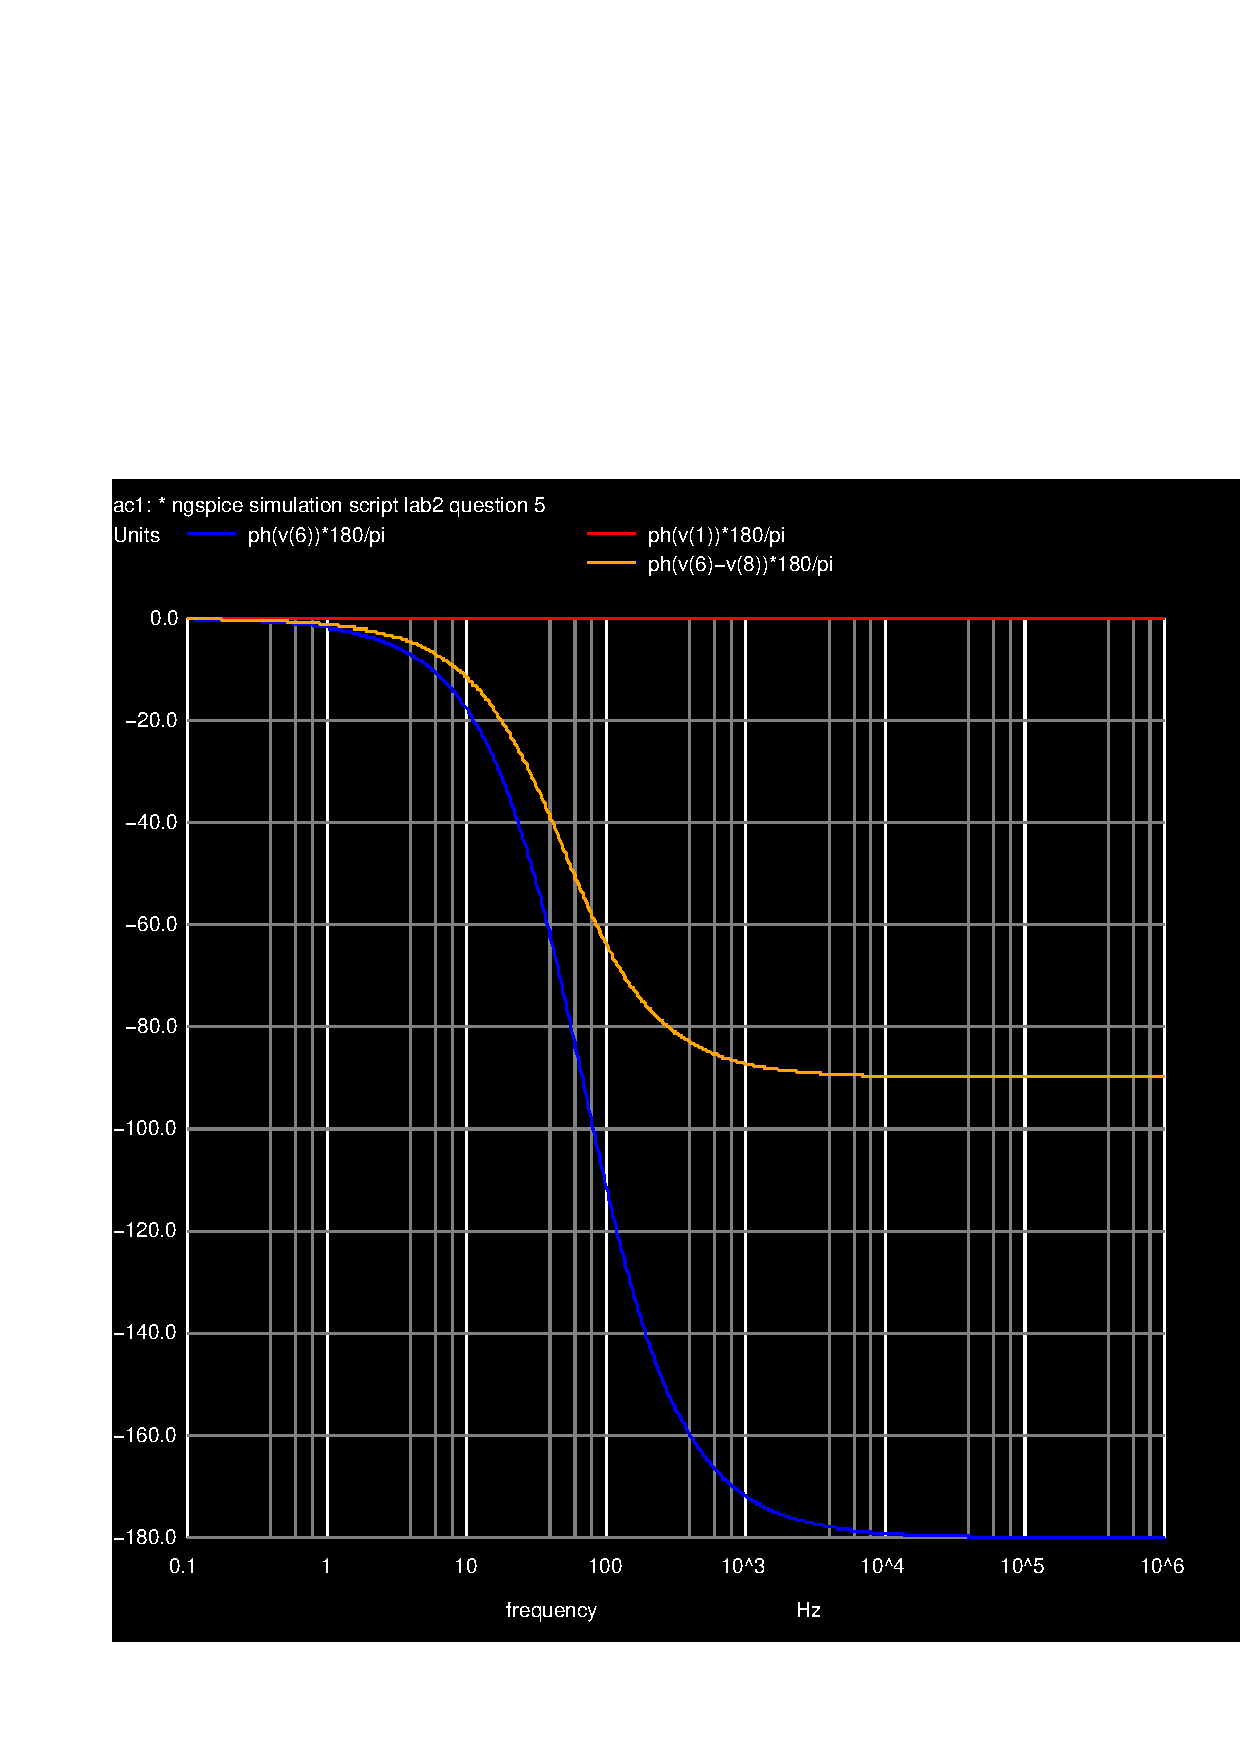
\includegraphics[width=0.9\linewidth]{sim5_ph.pdf}
\caption{Phase Response (in degrees)}
\label{fig:sim5_ph}
\end{figure}

\subsection{Comparison}
After comparing the graphics showed, it is clear to admit that the results in ngspice and octave fully match. As 
